\documentclass[11pt]{article}
\usepackage[final]{acl}
\usepackage{times}
\usepackage{amsmath}
\usepackage{latexsym}
\usepackage[T1]{fontenc}
\usepackage[utf8]{inputenc}
\usepackage{microtype}
\usepackage{inconsolata}
\usepackage{graphicx}

\title{Power Side Channel Analysis of Intel Processor}
\author{
    Himanshu Pandey \\
    Department of Computer Science\\
    Indian Institute of Technology Kanpur \\
    \texttt{phimanshu24@iitk.ac.in} \\
    \And
    Urbi Chatterjee \\
    Department of Computer Science\\
    Indian Institute of Technology Kanpur \\
    \texttt{urbic@iitk.ac.in} \\
}

\begin{document}
\maketitle

% Input files from Assignment2 subfolder
\begin{abstract}
Power side-channel attacks exploit variations in a processor’s energy consumption to extract secret information, posing a significant threat to secure computation in modern systems. In this work, we investigate the current feasibility of such attacks in light of industry-deployed mitigations, focusing on Intel’s post-PLATYPUS microcode updates and their effect on attack surface. We evaluate the persistence of side-channel leakage on an updated x86 platform by reproducing and extending PLATYPUS-style analyses, including instruction benchmarking, KASLR derandomization, and attacks on RSA exponentiation within an Intel SGX enclave.
Our findings confirm that disabling TSX via microcode effectively eliminates KASLR derandomization using power analysis. However, energy measurements obtained from the RAPL interface remain sufficiently sensitive to differentiate instruction types and operand Hamming weights, exposing a residual leakage channel. These results highlight that, despite microcode-level countermeasures, RAPL-based power side channels still threaten cryptographic operations in trusted execution environments. Ongoing research is necessary to develop robust defenses and accurately assess residual vulnerabilities in real-world platforms.\end{abstract}
\section{Introduction}
Modern processors achieve high performance through complex microarchitectural features designed to maximize instruction throughput. Two of the most significant are out-of-order execution and speculative execution. Instead of processing instructions in the strict, sequential order in which they appear in the program code, the CPU internally reorders them to execute instructions whose data is ready, rather than stalling on one that is waiting (e.g., for a slow memory access). Building on this, speculative execution allows
the CPU to predict the outcome of a conditional branch (e.g., an ‘if‘ statement) and begin execution of instructions from the predicted path before the condition is actually resolved \cite{8835233}.
These optimizations are managed by a deep pipeline of internal buffers and schedulers that are invisible to the programmer. If a prediction is correct, the results are committed to the architectural state (the registers and memory visible to the software), yielding a significant performance gain. If a prediction is wrong, the CPU discards the results from the incorrect path and starts over from the correct one. While the final architectural state remains correct, the act of transiently executing these mispredicted instructions is not without consequence. This transient execution can alter the processor’s underlying microarchitectural state—for instance, by loading data into a cache or training a branch
predictor. These changes create unintentional information flows known as side channels, which can be observed and exploited by an attacker to infer secret data \cite{3b07f496768442f48538a30b9f302940}.\\
To summarize, we make the following contributions:
\begin{enumerate}
\item We established a compatible hardware and software environment on a modern Intel CPU
running the latest microcode updates that disable TSX and obfuscate RAPL readings.
\item We determined that the instruction-level power signatures remain distinguishable through the
mitigated RAPL interface by replicating the instruction benchmarking experiments.
\item We investigated the potential for a privileged attack on an RSA implementation within
an SGX enclave by demonstrating that the foundational power leakage primitive
still exists post-mitigation.
\end{enumerate}
\textbf{Outline:} Section 2 presents a review of the foundational literature on related microarchitectural attacks and the core technologies enabling PLATYPUS. Section 3 details the methodology and specific configuration of the experimental setup. Section 4 presents the results from the reproduced experiments and discusses their
significance. We conclude in Section 5.
\section{Related Work}
Attempts to extract secrets from computational devices by observing indirect, uninten-
tional effects have been documented since World War II [1]. As computing advanced,
attacks exploiting these ”side channels” gradually found their way into cryptographic
research and security engineering. In the late 1990s, Kocher et al. demonstrated that
subtle variations in hardware power consumption could reveal cryptographic secrets, es-
tablishing the field of differential power analysis \cite{10.1007/3-540-48405-1_2}. This insight rapidly spurred research
into other physical side channels—electromagnetic emissions, timing measurements, and
even acoustic signals were shown to leak sensitive data, especially from cryptographic
algorithms.
Early side-channel attacks typically required an attacker with physical access, spe-
cialized equipment, and careful target profiling. Such constraints meant desktop-class
systems and servers were deemed relatively immune. This changed with the emergence
of microarchitectural attacks: researchers showed that features like branch prediction, speculative execution, and sophisticated cache hierarchies could leave measurable fingerprints that software alone could exploit \cite{8835233}\cite{3b07f496768442f48538a30b9f302940}. Today, side-channel attacks threaten nearly every class of modern computer, regardless of their physical security environment. 
\subsection{Power Side Channel Attacks}
Among physical side-channel vectors, power analysis occupies a prominent position due
to its direct relationship with transistor-level circuit activity . Any bit flip in digital
CMOS logic produces a measurable change in the processor’s power profile; the overall
power draw at a given cycle thus encodes both the current operation type and processed
data values. Power analysis was initially regarded as a hardware security threat confined to devices like smartcards or cryptographic accelerators, demanding direct probing and oscilloscopes for exploitation.
Recent advances have demonstrated, however, that software-accessible energy moni-
toring features in commodity processors offer sufficient resolution for attackers to infer
Instructive power traces are commonly used in power analysis. Equation~\ref{eq:Power_Consumption} presents the primary sources of power consumption, where $\alpha$ is the probability of a voltage transition, $C$ is the load capacitance, $V_{dd}$ is the supply voltage, $F$ is the clock frequency, $I_{\text{sc}}$ is the short-circuit current (when NMOS and PMOS transistors are active simultaneously), and $I_{\text{leak}}$ is the leakage current~\cite{371964}.


\begin{align}
P &= P_{\text{switching}} + (P_{\text{short-circuit}} + P_{\text{leakage}}) \nonumber \\
  &= \alpha \cdot C \cdot V_{dd}^2 \cdot F + I_{\text{sc}} \cdot V_{dd} + I_{\text{leak}} \cdot V_{dd}
  \label{eq:Power_Consumption}
\end{align}
For instance, energy readouts and update rate of the energy counters varies by domain and microarchitecture which are typically computed using \( E_{\text{joules}} = \text{Raw}_{\text{Value}} \times \text{Energy Unit (Joules)} \).

\subsection{Variants of Power Analysis}
Power side-channel attacks exploit the fact that the power consumption of a processor’s CMOS circuits is data-dependent. The instantaneous power consumption of a circuit can be divided into static and dynamic components. While static power is due to leakage currents, dynamic power is consumed during state transitions, such as when transistors switch from 0 to 1 or vice versa. This switching power is significantly larger than other components and is directly influenced by the data being processed and the operation being performed. An attacker can measure these variations to deduce secret information.
\subsubsection{Simple Power Analysis (SPA)}
Simple Powe Analysis involves visually or algorithmically analyzing single or small sets of power consumption traces to identify large-scale differences that correspond to specific operations or code paths~\cite{10.1007/3-540-48405-1_2}. For example, the classic square-
and-multiply implementation of RSA can leak the secret key if a squaring operation is always performed, but an additional multiply operation only occurs for key bits set to ’1’. This difference creates detectable power patterns, allowing attackers to deduce secret bits from a handful of traces. While SPA is powerful when implementation differences are pronounced and measurement noise is low, it can often be mitigated by enforcing strictly uniform operation sequences~\cite{10.1007/3-540-48405-1_2}.
\subsubsection{Differential Power Analysis (DPA)}
Differential Power Analysis uses statistical methods to amplify small variations in power consumption that correlate with secret data~\cite{10.1007/3-540-48405-1_2}. An attacker collects a large number of power traces while the device processes a number of varying, but
known, inputs. By partitioning traces based on a hypothesis about internal computation (such as a key bit or byte), and then comparing the average power consumption of each partition, data-independent effects and random noise are averaged out, while subtler, data-dependent differences are exposed. DPA dramatically expands the range
of exploitable leakages, working even when SPA fails, and poses a threat to nearly all 
cryptographic implementations not designed with side channels in mind.
\subsubsection{Correlation Power Analysis}
Correlation Power Analysis (CPA) builds on the DPA methodology by incorporating explicit leakage models. Instead of merely comparing averages, attackers hypothesize intermediate computation values (e.g., the output of an S-box or register value during encryption) and use a model—such as the Hamming weight or Hamming distance to
predict the device’s power consumption for each guess. For each candidate key, a vector of predicted power values is generated and compared with the actual measured power traces using the Pearson correlation coefficient—a statistical measure of linear dependence between two variables. The key candidate with the highest correlation value is considered the most likely to be correct~\cite{10.1007/978-3-540-28632-5_2}. By leveraging statistical correlation, CPA can reveal subtle, systematic leakage that might elude simpler analyses, making it a standard and powerful technique for practical side-channel cryptanalysis. To recover a secret value, we compute the correlation $\rho(p, h)$ between the observed power consumptions $p_n$ and hypothetical leakage values $h_n$ over all $N$ traces. The choice of $h$ depends on the targeted operation and the leakage characteristics of the target implementation and processor. 

For example, for recovering byte 0 of the round key in the final round of AES, a common choice (given a key candidate $k$) is:
\begin{equation}
h^k_n = HW\left(SBox^{-1}\left(c^0_n \oplus k\right)\right)
\end{equation}
where $c^0_n$ is byte 0 of the $n$th ciphertext, and $HW$ denotes the Hamming weight. Computing $\rho_k(p, h^k)$ for all candidates $k = 0 \dots 255$, the correct key candidate can be identified as the one with maximum correlation. This process is repeated for each byte. 

Other choices of $h$ are possible, e.g., when targeting the XOR in the first round of AES:
\begin{equation}
h^k_n = HW\left(x^0_n \oplus k\right)
\end{equation}

For a given number of traces $N$, the noise level is:
\begin{equation}
\rho_{\text{noise}} = \frac{4}{\sqrt{N}}
\end{equation}
Only correlations $\rho \geq \rho_{\text{noise}}$ are considered significant.


\section{Intel RAPL Leakage Analysis}
Intel Software Guard Extensions (SGX) is an architectural extension of x86 processors
designed to provide secure, isolated execution environments known as enclaves. Enclaves
are regions of application memory where code and data are protected by hardware from
all other software on the system, including the operating system, hypervisor, and even the
system BIOS. The core security guarantee is that even if the rest of the platform is fully
compromised, enclave memory contents remain confidential and tamper-resistant.
When a process creates an enclave, the memory pages assigned to it are designated as
special by the SGX hardware. Accesses to this range are permitted only during enclave
mode; any access attempt by non-enclave code, regardless of privilege level, is blocked.
This is enforced by checks at the CPU’s memory controller, effectively preventing even
kernel or DMA attacks. 
\begin{figure}
    \centering
    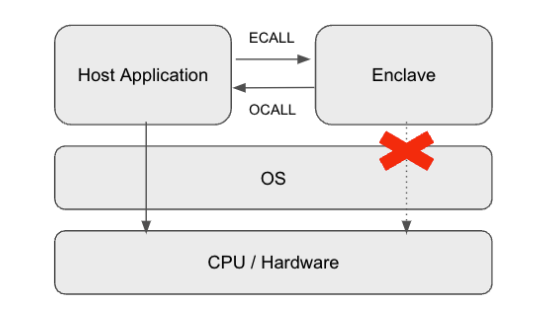
\includegraphics[width=0.8\linewidth]{Assignment2- Writing a Research Paper in Latex/Images/Intel_SGX.png}
    \caption{Organization of Intel SGX}
    \label{fig:Intel_SGX}
\end{figure}
Organization of protected memory regions in Intel SGX is shown in Figure \ref{fig:Intel_SGX}. Enclave code and data are inaccessible to the OS and all other non-enclave software.
\section{Results}
\begin{figure}[h]
    \centering
    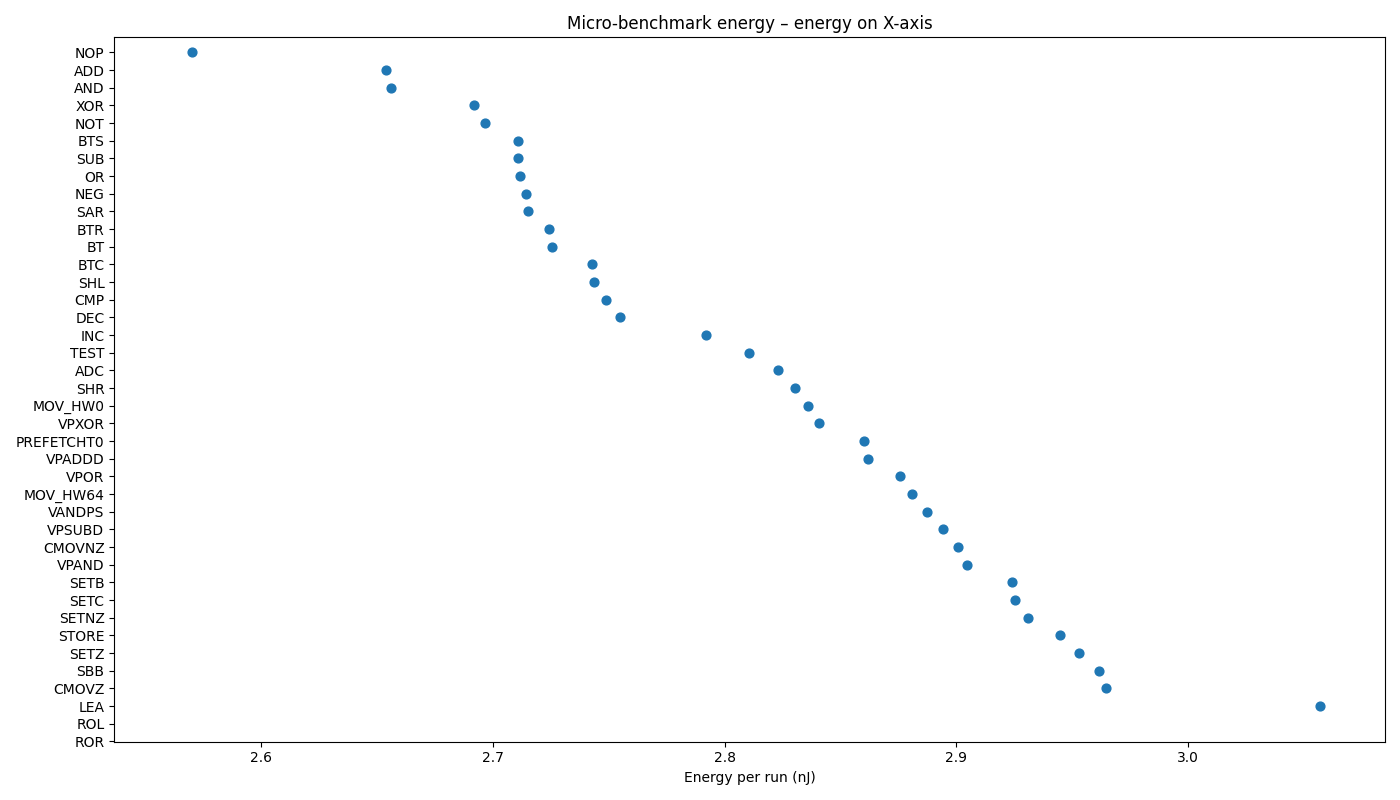
\includegraphics[width=1\linewidth]{Assignment2- Writing a Research Paper in Latex/Images/Instructions_Energy_Readings.png}
    \caption{Energy Consumption Profile of Various x86 Instructions. Each point represents
the energy consumed per run (total/5B) in nJ}
    \label{fig:Instructions_Energy_Readings}
\end{figure}

\begin{table*}[!t]
  \centering
  \begin{tabular}{lccccc}
    \hline
    \textbf{Instruction} & \textbf{Xeon Silver 4214} & \textbf{i7-6700K} & \textbf{i7-8650U} & \textbf{i5-8250U} & \textbf{Xeon Gold 6248} \\
    \hline
    nop                & 0.1795 nJ & 0.1189 nJ & 0.0843 nJ & 0.0912 nJ & 0.1768 nJ \\
    inc r64            & 0.1795 nJ & 0.1208 nJ & 0.0858 nJ & 0.0931 nJ & 0.1781 nJ \\
    xor r64, r64       & 0.1795 nJ & 0.1209 nJ & 0.0849 nJ & 0.0924 nJ & 0.1774 nJ \\
    mov r64, mem       & 0.1868 nJ & 0.1247 nJ & 0.0840 nJ & 0.0950 nJ & 0.1839 nJ \\
    imul r64, r64      & 0.1798 nJ & 0.1169 nJ & 0.0887 nJ & 0.0942 nJ & 0.1792 nJ \\
    fscale             & 0.1867 nJ & 0.1182 nJ & 0.0877 nJ & 0.0963 nJ & 0.1845 nJ \\
    rdrand r64         & 0.1797 nJ & 0.1129 nJ & 0.0982 nJ & 0.1047 nJ & 0.1801 nJ \\
    rdtsc              & 0.1864 nJ & 0.1189 nJ & 0.0848 nJ & 0.0929 nJ & 0.1835 nJ \\
    clflush mem        & 0.1865 nJ & 0.1129 nJ & 0.1018 nJ & 0.1085 nJ & 0.1851 nJ \\
    aesenc xmm, xmm    & 0.1794 nJ & 0.1188 nJ & 0.0946 nJ & 0.1012 nJ & 0.1790 nJ \\
    \hline
  \end{tabular}
  \caption{Per-instruction energy consumption for different Intel processors.
  }
  \label{table:instruction-energy}
\end{table*}

The first and most fundamental experiment was to verify if the foundational leakage pattern of the PLATYPUS attack still exists on a modern, patched processor. The objective was to determine whether the power consumption of different x86 instructions remain distinguishable through the mitigated RAPL interface. If the mitigations were completely effective, we would expect the power consumption to be uniform or for the added noise to overwhelm any signal. We benchmarked 69 instructions for this experiment. We also benchmarked the effect of Hamming Weight on the power consumption of an instruction.

The results strongly suggest that Intel’s RAPL obfuscation, while adding noise,
is insufficient to mask the power variations caused by different CPU operations completely. The data, visualized in Figure \ref{fig:Instructions_Energy_Readings}, reveals a distinct and hierarchical energy profile.
Table \ref{table:instruction-energy} lists the measured energy consumption of different
instructions on our i7-6700K (desktop), Xeon Silver 4214 (server), and i7-8650U (mobile) systems, i5-8250U and Xeon Gold6248. We can clearly
observe inter-instruction differences in energy consumption.
\section{Conclusion}
This work presents a systematic investigation of the modern attack surface posed by
software-based power side channels on post-mitigation Intel x86 platforms, with a focus on the efficacy of vendor-deployed countermeasures following the publication of the PLATYPUS attack. Through detailed replication and extension of foundational experiments, we have confirmed that while certain attack vectors—most notably TSX-assisted KASLR derandomization—are effectively neutralized by recent microcode updates, other forms of leakage persist.
Specifically, we demonstrated that, even in the presence of energy obfuscation and
access restrictions, the Intel RAPL interface continues to expose coarse-grained but distinguishable power signatures for different instructions and data values. Instruction-level energy differences and operand Hamming weights remain measurable, with implications for the security of cryptographic operations. Our experiments further validated the continued vulnerability of RSA modular exponentiation within SGX enclaves: power usage remains highly dependent on secret key material, and RAPL can differentiate between low- and high-entropy keys even after all countermeasures are deployed.
These findings reinforce that software-accessible power side channels, though blunted, cannot be fully eliminated by microcode-based noise injection or interface gating alone. Ongoing research and a careful re-evaluation of trusted execution environment threat models are needed to close the remaining gaps.

% Bibliography path relative to CS888.tex root
\bibliographystyle{plain}
\bibliography{custom}

\appendix
\section{Appendix}
\label{sec:appendix}
While we focus on Intel’s RAPL implementation throughout this work, other microarchitectures offer different interfaces to obtain the energy consumption of the core.
AMD: Since the Zen (family 17H)  microarchitecture, AMD CPUs have provided a RAPL interface [2]. However, little documentation is available regarding its implementation. 
Power consumption values for the core and package domains are provided respectively in the CORE\_ENERGY\_STAT and
PKG\_ENERGY\_STAT MSRs. A notable difference from Intel RAPL is that the core domain is accessible per-core rather than across all cores of the CPU, which substantially reduces
measurement noise. An attacker targeting AMD currently requires root privileges to read the MSRs, as the Linux powercap driver
only establishes a user-accessible sysfs RAPL interface on Intel CPUs. While they lack the RAPL interface, earlier AMD family 15h and 16h CPUs also have power MSRs which provide consumption estimates based on platform activity levels. Unfortunately, none were available to us for evaluation purposes. However, we believe systems with these
CPUs may be vulnerable to user-space attacks because if the fam15h\_power driver is loaded, power values can be read from user space via sysfs.


\end{document}
